\documentclass[11pt]{article}

% URLs and hyperlinks ---------------------------------------
\usepackage{hyperref}
\hypersetup{
    colorlinks=true,
    linkcolor=blue,
    filecolor=magenta,      
    urlcolor=black,
}
\usepackage{xurl}
%---------------------------------------------------

\usepackage{amsmath}
\usepackage{float}
\usepackage{graphicx}
% footnotes in headings -------------------------------------
\usepackage[stable]{footmisc}
%------------------------------------------------------------

\usepackage{float}

\usepackage{xepersian}
\settextfont{Yas}
\setdigitfont{Yas}

\newcommand{\mahdi}{مهدی حق‌وردی }
\newcommand{\hosna}{حسنا رجایی }

\title{پاسخ تمرینات فصل اول - مقدمات و \lr{Performance}}
\author{
    حسنا رجایی \\
    مهدی‌ حق‌وردی}
\date{}

\begin{document}
\maketitle    
\section{}
\begin{center}
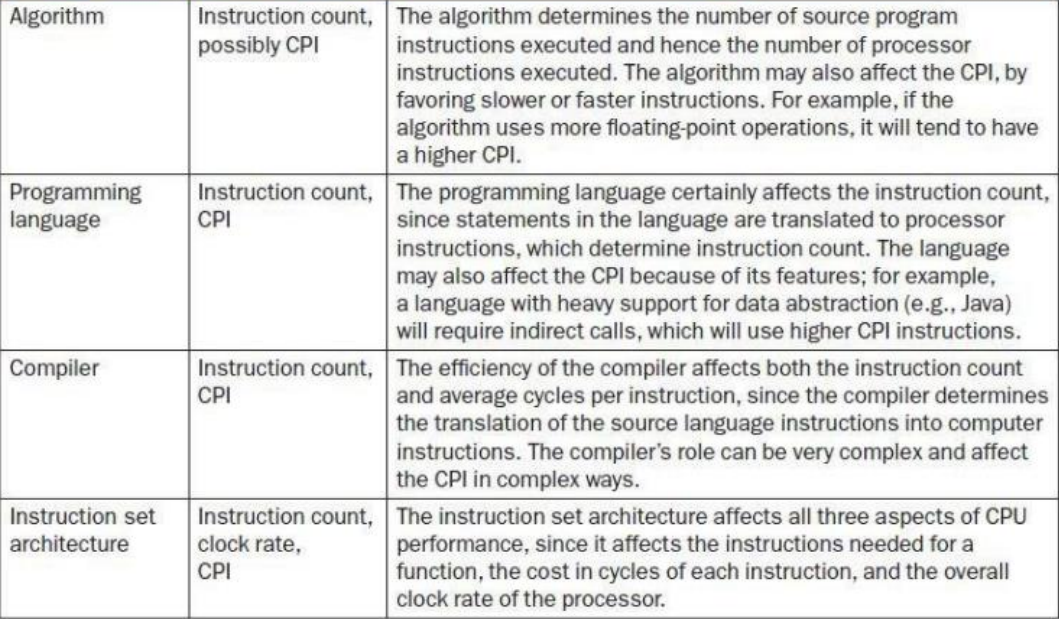
\includegraphics[width=0.7\textwidth, height=0.4\textheight]{1}
\end{center}

\section{}
\subsection{}
\begin{latin}
Instr/sec = f/CPI

\begin{itemize}
    \item 
    $P1 = \frac{3}{1.5} \times 10^9 = 2 \times 10^9$
    \item 
    $P2 = \frac{2.5}{1.0} \times 10^9 = 2.5 \times 10^9$
    \item 
    $P3 = \frac{4}{2.2} \times 10^9 = 1.8 \times 10^9$
\end{itemize}
\end{latin}

\subsection{}
\begin{latin}
\indent \indent Formulas:
\begin{itemize}
\item No. cycles = time $\times$ clock rate
\item time = (No. Instr $\times$ CPI)/clock rate \item No. instructions = No. cycles/CPI
\end{itemize}

Answers:
\begin{itemize}
\item P1

cycles = $10 \times 3 \times 10^9 = 30 \times 10^9$ s

No. instructions = $\frac{30}{1.5} \times 10^9 = 20 \times 10^9$

\item P2

cycles = $10 \times 2.5 \times 10^9 = 25 \times 10^9$ s

No. instructions = $\frac{25}{1.0} \times 10^9 = 25 \times 10^9$

\item P3

cycles = $10 \times 4 \times 10^9 = 40 \times 10^9$ s

No. instructions = $\frac{40}{2.2} \times 10^9 = 18.18 \times 10^9$

\end{itemize}
\end{latin}

\subsection{}
\begin{latin}
\indent \indent $\text{time}_{\text{new}} = \text{time}_{\text{old}} \times 0.7 = 7$ s

$\text{CPI}_{\text{new}} = \text{CPI}_{\text{old}} \times 1.2 \Rightarrow \text{CPI(P1)} = 1.8, \text{CPI(P2)} = 1.2, \text{CPI(P3)} = 2.6$

f = No. Instr $\times$ CPI/time

\begin{itemize}
    \item P1 $\rightarrow 20 \times 10^9 \times \frac{1.8}{7} = 5.14 \ \text{GHz}$
    \item P2 $\rightarrow 25 \times 10^9 \times \frac{1.2}{7} = 4.28 \ \text{GHz}$
    \item P3 $\rightarrow 18.18 \times 10^9 \times \frac{2.6}{7} = 6.75 \ \text{GHz}$    
\end{itemize}
\end{latin}

\section{}
\subsection{}
\begin{latin}
Class A: $10^6$ instr. \\
Class B: 2 $\times 10^6$ instr.\\
Class C: 5 $\times 10^6$ instr.\\
Class D: 2 $\times 10^6$ instr.\\
Time = No. instr $\times$ CPI/clock rate

\begin{itemize}
    \item P1 $$\frac{(10^6) + (2 \times 10^6 \times 2) + (5 \times 10^6 \times 3) + (2 \times 10^6 \times 3)}{2.5 \times 10^9} = 10.4 \times 10^{-3} \ \text{s}$$
    
    \item P2 $$\frac{(10^6 \times 2) + (2 \times 10^6 \times 2) + (5 \times 10^6 \times 2) + (2 \times 10^6 \times 2)}{3 \times 10^9} = 6.66 \times 10^{-3} \ \text{s}$$
\end{itemize}
\end{latin}

\subsection{}
\begin{latin}
CPI = time $\times$ clock rate/No. instr

\begin{itemize}
    \item P1 = $10.4 \times 10^{-3} \times \frac{2.5 \times 10^9}{10^6} = 26$
    \item P2 = $6.66 \times 10^{-3} \times \frac{3 \times 10^9}{10^6} = 20$
\end{itemize}
\end{latin}

\subsection{}
\begin{latin}

\begin{itemize}
\item P1 = $(10^6 \times 1) + (2 \times 10^6 \times 2) + (5 \times 10^6 \times 3) + (2 \times 10^6 \times 3) = 26 \times 10^6$

\item P2 = $(10^6 \times 2) + (2 \times 10^6 \times 2) + (5 \times 10^6 \times 2) + (2 \times 10^6 \times 2) = 20 \times 10^6$

\end{itemize}
\end{latin}
\section{}
\subsection{}
\begin{latin}
No. Instr = CPU time $\times$ Clock rate / CPI

\begin{itemize}
    \item A $\rightarrow 820 \times 0.9 \times 4 \times \frac{10^9}{0.96} = 3075 \times 10^9$
    
    \item B $\rightarrow 580 \times 0.9 \times 4 \times \frac{10^9}{2.94} = 710 \times 10^9$
\end{itemize}
\end{latin}

\subsection{}
\begin{latin}
\indent \indent Clock rate = No. Instr $\times$ CPI/CPU time

$\text{Clock rate}_{\text{new}} = \text{No. Instr} \times \frac{\text{CPI}}{0.9} \times \text{CPU time} \Rightarrow \frac{1}{0.9} \times \text{Clock rate}_{\text{old}} = 3.33 \ \text{GHz}$
\end{latin}

\subsection{}
\begin{latin}
\indent \indent Clock rate = No. Instr $times$ CPI/CPU time

$\text{Clock rate}_{\text{new}} = \text{No. Instr} \times 0.85 \times \frac{\text{CPI}}{0.80} \times \text{CPU time} \Rightarrow \frac{0.85}{0.80} \times \text{Clock rate}_{\text{old}} = 3.18 \ \text{GHz}$
\end{latin}

\section{}
\subsection{}
\begin{latin}
\indent \indent CPI = clock rate $\times$ CPU time/instr count

\begin{itemize}
    \item CPI(bzip2) = $3 \times 10^9 \times \frac{750}{2389 \times 10^9} = 0.94$
    
    \item CPI(go) = $3 \times 10^9 \times \frac{700}{1658 \times 10^9} = 1.26$
\end{itemize}
\end{latin}

\subsection{}
\begin{latin}
\indent \indent CPU time = No. instr × CPI/clock rate

If CPI and clock rate do not change, the CPU time increase is equal to the increase in the of number of instructions, that is, 10\%.
\end{latin}

\subsection{}
\begin{latin}
\indent \indent CPU time(before) = No. instr $\times$ CPI/clock rate

CPU time(after) = 1.1 $\times$ No. instr $\times$ 1.05 $\times$ CPI/clock rate

CPU times(after)/CPU time(before) = 1.1 $\times$ 1.05 = 1.155 Thus, CPU time is
increased by 15.5\%.
\end{latin}
\end{document}